\documentclass[english,hidelinks,pdftex, 11 pt, class=report,crop=false]{standalone}
\usepackage[T1]{fontenc}
\usepackage[utf8]{luainputenc}
\usepackage{geometry}
\geometry{verbose,paperwidth=16.4 cm, paperheight=29cm, inner=1.5cm, outer=1.5 cm, bmargin=1.5cm, tmargin=1.5cm}
\usepackage{import}
\usepackage[subpreambles=false]{standalone}
\usepackage{amsmath}
\usepackage{amssymb}
\usepackage{esint}
\usepackage{babel}
\usepackage{tabu}
\setlength{\parindent}{0bp}
\usepackage{enumitem}
\usepackage{xcolor}

\begin{document}
\huge \textbf{Lekseark matematikk fredag} \\[25pt]
\large
\textit{\textbf{Før svara fint inn i rekneboka di.}} \\[15pt]
{\Large \textbf{Oppgåve 1}}\\[10pt]
Rekn ut. Du \textbf{skal} vise utrekning. Sjekk svara dine med kalkulator før du leverer, og rett opp viss du har gjort feil. \\[10pt]
\textbf{a)} $ 48\cdot3 $\qquad \textbf{b)} $ 29\cdot6 $\qquad \textbf{c)} $ 702\cdot8 $\\[12pt]
\textbf{d)} $ 256\cdot3 $\qquad \textbf{e)} $ 24\cdot 17 $\qquad \textbf{f)} $ 129\cdot 34 $ \vspace{30pt}

{\Large \textbf{Oppgåve 2}}\\[10pt]
Rekn ut. Du \textbf{skal} vise utrekning. Sjekk svara dine med kalkulator før du leverer og rett opp viss du har gjort feil. \\[10pt]
\textbf{a)} $ 96:4 $\qquad \textbf{b)} $ 54:3  $\qquad \textbf{c)} $ 162:6 $\\[12pt]
\textbf{d)} $ 875:7 $\qquad \textbf{e)} $ 1384:8$\qquad \textbf{f)} $ 1827:9  $
\begin{center}
	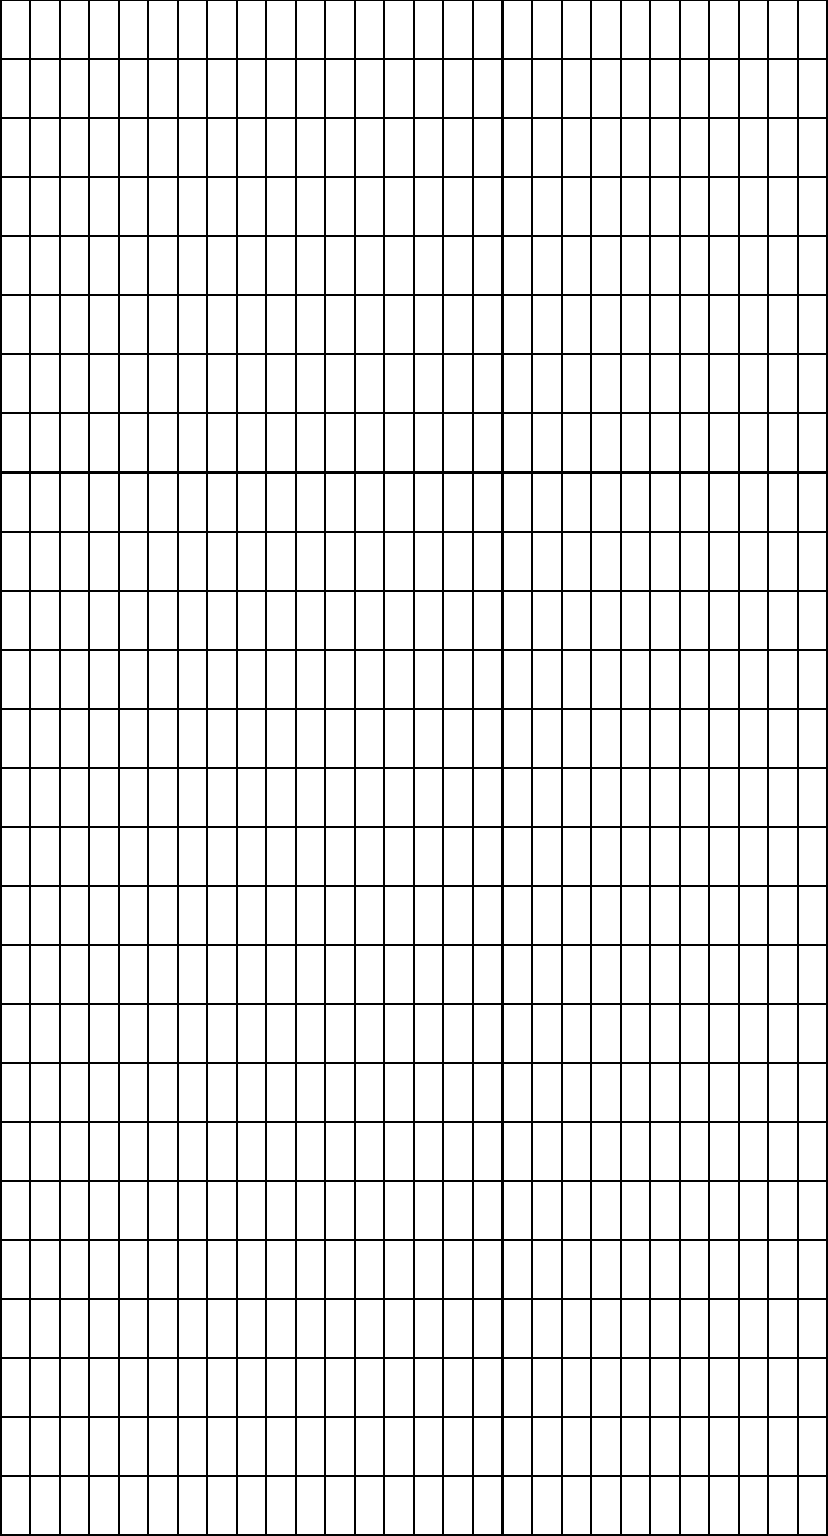
\includegraphics[]{sheet}
\end{center}
\end{document}

